\documentclass[12pt,a4paper]{article}

\usepackage[utf8]{inputenc}
\usepackage{graphicx}
\usepackage{float}

\begin{document}

\title{MI-PAA 2015 1.ukol}
\author{Tomas Nesrovnal\\nesrotom@fit.cvut.cz}
\date{\today}
\maketitle

\section{Specifikace ulohy}
Problem 0-1 batohu.

\section{Rozbor moznych variant reseni}
Ulohu muzu resit hrubou silou. Ziskam tam presny vysledek, ale vypocet bude
pomaly. Dalsim resenim je pouzit heuristiku, jejiz vyledek nebude nejlepsi mozny
ale vypocet probehne rychle.

\section{Ramcovy popis postupu reseni}
\subsection{Hruba sila}
Zkusim vsechny moznosti a vyberu tu nejlepsi.
\subsection{Heuristika}
Vkladam do bahothu nejlepsi predmety s pomerem cena/vaha, dokud
mi jeste staci kapacita.

\section{Popis kostry algoritmu}
\subsection{Hruba sila}
Vytvorim pole, ktere udava ktery predmet je v batohu. Rekurzivne zkousim
vsechny moznosti (zavolam rekurzi bez prvku, pak prvek pridam a zavolam rekurzi znovu).
Ulozim si nejlepsi reseni.

Druha varianta obsahuje vylepseni: Pokud ve stromu reseni narazim na to, ze se do batohu uz vic nevejde, vetev zariznu.
\subsection{Heuristika}
Seradim si pole s predmety podle pomeru cena/vaha (nebo jine varianty, viz grafy). Cele pole sestupne prochazim a pokud se tam predmet vejde, tak ho tam vlozim.

\section{Namerene vysledky}

\subsection{Spravnost vysledku}
Pomoci skriptu byla overena spravnost vysledku (porovnanim s referencnim resenim).

\subsection{Na cem bylo mereno}
Intel(R) Core(TM) i3-2328M Processor (3M Cache, 2.20 GHz), gcc 4.9.2 (-Ofast), OS GNU/Linux Lubuntu 14.04 64bit

\subsection{Grafy}
Vsechny grafy byly vygenerovany skriptem (error.sh). Cas byl meren pomoci knihovny OpenMPI.
Sript byl spusten pres prikaz \textbf{sudo time nice -n -20 ./error.sh} a trval 180 sekund.

Presna cisla lze nalezt v \textbf{*.plot} souborech.

Chyba heuristiky: Z kazdeho batohu spocitana relativni chyba. V grafu jsou pak secteny relativni chyby pro celou sadu. Celkem 3 heuristiky.

\begin{figure}[H]
	\caption{Doba behu reseni heuristikou (cena/vaha). 5000 opakovani. }
	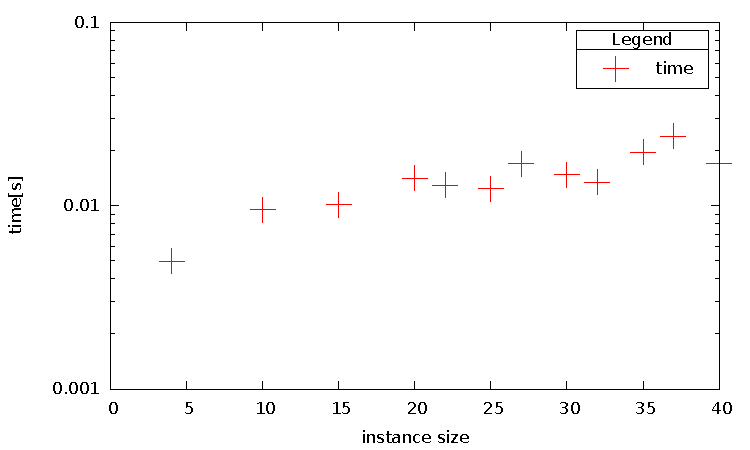
\includegraphics{./time_h1.pdf}
\end{figure}

\begin{figure}[H]
	\caption{Doba behu reseni hrubou silou. 5 opakovani. }
	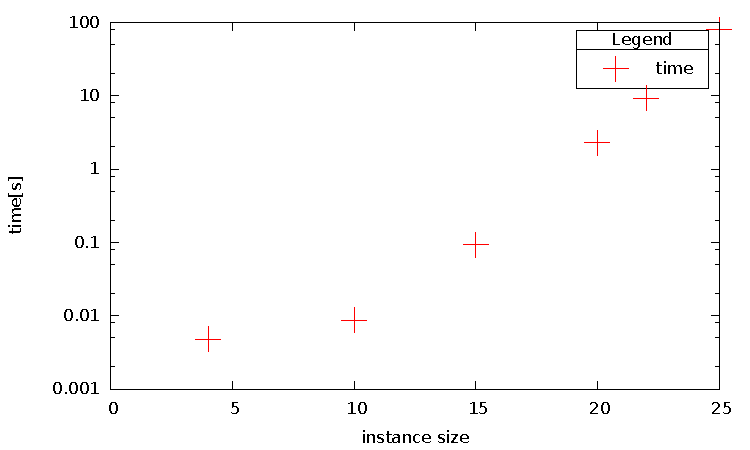
\includegraphics{./time_b0.pdf}
\end{figure}

\begin{figure}[H]
	\caption{Doba behu reseni hrubou silou (s orezavanim). 5 opakovani. }
	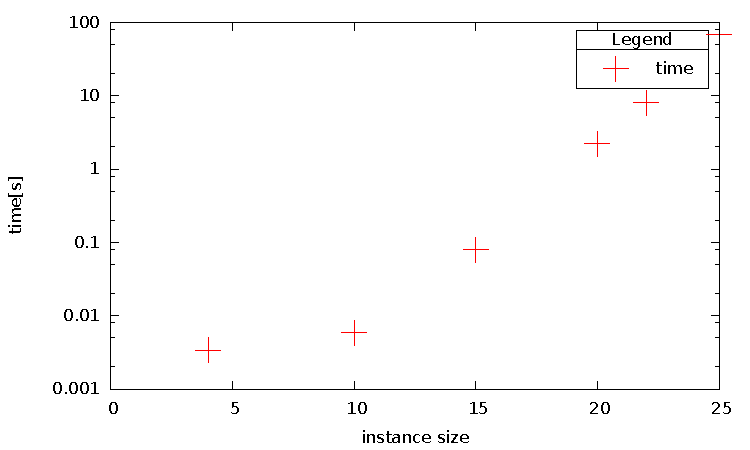
\includegraphics{./time_b1.pdf}
\end{figure}

\begin{figure}[H]
	\caption{heuristika (podle ceho se radilo): pomer cena/vaha}
	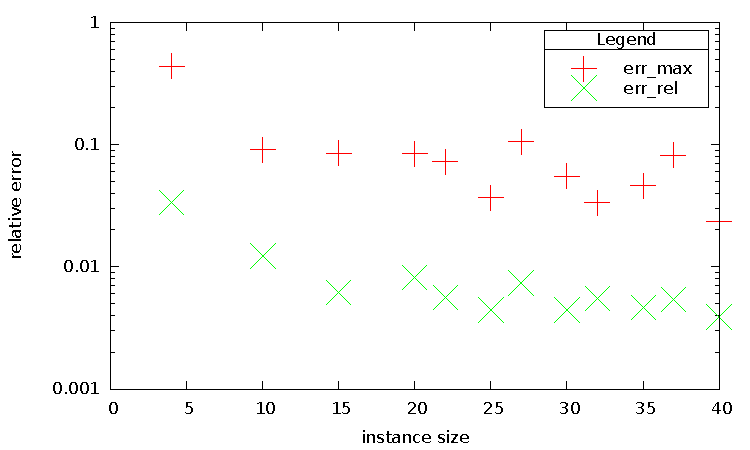
\includegraphics{./err_h1.pdf}
\end{figure}

\begin{figure}[H]
	\caption{heuristika (podle ceho se radilo): cena}
	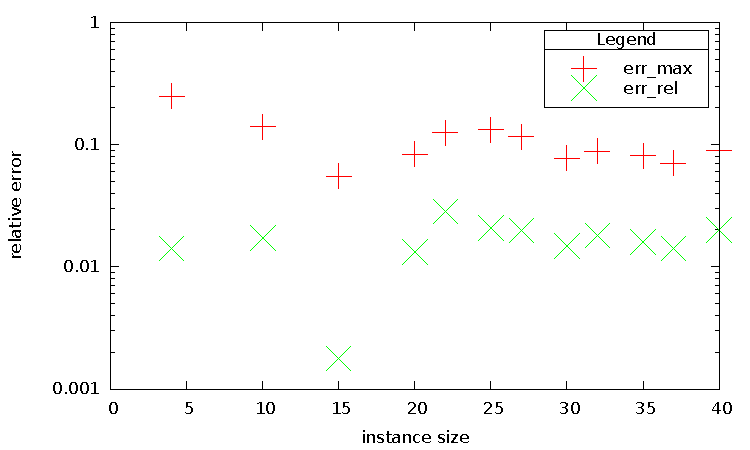
\includegraphics{./err_h2.pdf}
\end{figure}

\begin{figure}[H]
	\caption{heuristika (podle ceho se radilo): vaha}
	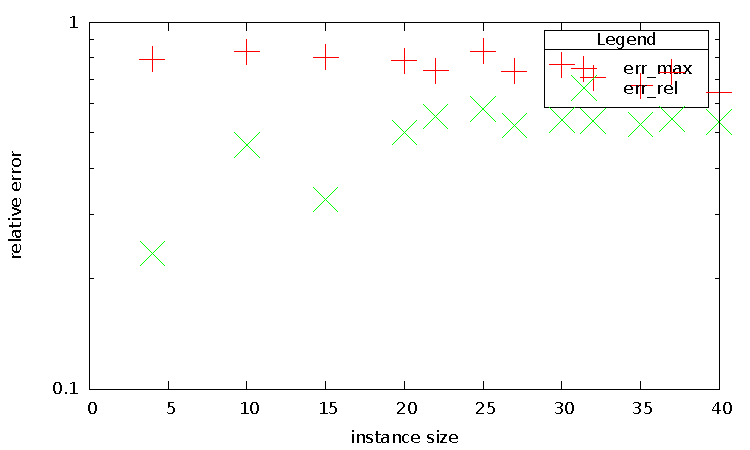
\includegraphics{./err_h3.pdf}
\end{figure}


\section{Zaver}
Vysledky se shoduji s rozborem reseni. Hruba sila je opravdu pomala a byt jednoducha heuristika nevraci zas tak spatne reseni.

Heuristika cena/vaha byla nejlepsi z heuristik.

Orezavani bruteforce melo za nasledek zrychleni o 12 sekund u instance o velikosti 25.

Bruteforce ma slozitost \textbf{O(n!)}, zatimco heuristika jen \textbf{O(nlogn)}. Z tohoto duvodu bylo mereni na heuristice opakovano 50000x, zatimco na bruteforce pouze 5x.

Jeste nutno podotknout, ze na takhle malych datech (navic asi nahodne vygenerovanych) muzou byt velke odchylky a anomalie.
\end{document}
